\documentclass{article}

\usepackage{xcolor}
\usepackage{hyperref}
\definecolor{COLOR_MEAN}{HTML}{f0f0f0}
\definecolor{LINK_COLOR}{HTML}{636EFA}
\hypersetup{
	colorlinks=true,
	linkcolor=LINK_COLOR,
	urlcolor=LINK_COLOR,
	citecolor=LINK_COLOR,
}

% if you need to pass options to natbib, use, e.g.:
%     \PassOptionsToPackage{numbers, compress}{natbib}
% before loading neurips_2024


% ready for submission
%\usepackage{neurips_2024}


% to compile a preprint version, e.g., for submission to arXiv, add add the
% [preprint] option:
% \usepackage[preprint]{neurips_2024}


% to compile a camera-ready version, add the [final] option, e.g.:
\usepackage[final]{neurips_2024}


% to avoid loading the natbib package, add option nonatbib:
%    \usepackage[nonatbib]{neurips_2024}


\usepackage[utf8]{inputenc} % allow utf-8 input
\usepackage[T1]{fontenc}    % use 8-bit T1 fonts
\usepackage{hyperref}       % hyperlinks
\usepackage{url}            % simple URL typesetting
\usepackage{booktabs}       % professional-quality tables
\usepackage{amsfonts}       % blackboard math symbols
\usepackage{nicefrac}       % compact symbols for 1/2, etc.
\usepackage{microtype}      % microtypography
\usepackage{xcolor}         % colors
\usepackage{tabularx}
\usepackage{booktabs}
\usepackage{amsmath}
\usepackage{listings}
\usepackage{tikz}



\title{MH4320 Assignment 2}


% The \author macro works with any number of authors. There are two commands
% used to separate the names and addresses of multiple authors: \And and \AND.
%
% Using \And between authors leaves it to LaTeX to determine where to break the
% lines. Using \AND forces a line break at that point. So, if LaTeX puts 3 of 4
% authors names on the first line, and the last on the second line, try using
% \AND instead of \And before the third author name.


\author{%
	Pu Fanyi \\
	College of Computing and Data Science\\
	Nanyang Technological University\\
	Singapore 639798 \\
	\texttt{FPU001@e.ntu.edu.sg} \\
}

\usepackage{graphicx}

\begin{document}
	
	
	\maketitle	
	
	\section{Football Penalty Kick}

    \subsection{Mixed Nash Equilibrium}

    \label{sec:football}

    Let Kicker plays ``Left'' with probability $\alpha$ and ``Right'' with probability $1-\alpha$. At the same time, Goalie plays ``Left'' with probability $\beta$ and ``Right'' with probability $1-\beta$.

    We define $b_K(\beta_0)$ be the set of best responses ($\alpha$) for Kicker when $\beta=\beta_0$, and $b_G(\alpha_0)$ be the set of best responses ($\beta$) for Goalie when $\alpha=\alpha_0$. And we define $U_K(\alpha_0, \beta_0), U_G(\alpha_0, \beta_0)$ as the expected utility they earned when $\alpha=\alpha_0, \beta=\beta_0$.

    We have:
    \begin{align*}
    U_K(\alpha, \beta) &= \alpha\cdot(1-\beta)+(1-\alpha)\cdot\beta\\
    &=\alpha+\beta-2\alpha\beta\\
    &=\beta+(1-2\beta)\cdot\alpha\\
    U_G(\alpha, \beta)&=\alpha\beta+(1-\alpha)(1-\beta)\\
    &=2\alpha\beta-\alpha-\beta+1\\
    &=(2\alpha-1)\beta-\alpha+1
    \end{align*}

    As $U_K(\alpha), U_G(\beta)$ are linear functions, we can know that:
    \begin{align*}
        b_K(\beta)=\begin{cases}
            \{1\}&\beta<\frac{1}{2}\\
            [0, 1]&\beta=\frac{1}{2}\\
            \{0\}&\beta>\frac{1}{2}
        \end{cases}\\
        b_G(\alpha)=\begin{cases}
            \{0\}&\alpha<\frac{1}{2}\\
            [0, 1]&\alpha=\frac{1}{2}\\
            \{1\}&\alpha>\frac{1}{2}
        \end{cases}
    \end{align*}

    If $\left<\alpha, \beta\right>$ is an NE, we can know that:
    $$
    \begin{cases}
        \alpha\in b_K(\beta)\\
        \beta\in b_G(\alpha)
    \end{cases}
    $$

    We can draw $(\beta, b_K(\beta))$ and $(\alpha, b_G(\alpha))$ on a single $\alpha$-$\beta$ plane to solve this equation, as shown in Figure~\ref{fig:best_response_1_1}.
    
    \begin{figure}[t]
    \centering
     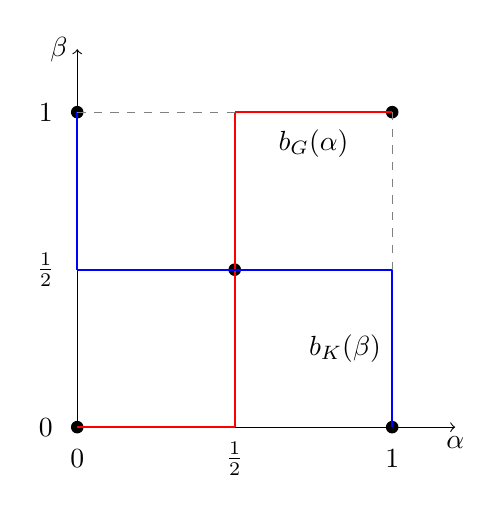
\begin{tikzpicture}[scale=4]
            % Axes
            \draw[->] (0,0) -- (1.2,0) node[below] {$\alpha$};
            \draw[->] (0,0) -- (0,1.2) node[left] {$\beta$};
        
            % Points
            \fill (0,0) circle (0.02); 
            \fill (0,1) circle (0.02); 
            \fill (1,0) circle (0.02); 
            \fill (1,1) circle (0.02); 
            \fill (0.5,0.5) circle (0.02); 
        
            % Lines for best responses
            \draw[thick, blue] (0,1) -- (0, 0.5);
            \draw[thick, red] (0,0) -- (0.5,0);
            \draw[thick, red] (0.5,0) -- (0.5,1);
            \draw[thick, blue] (1,0) -- (1, 0.5);
            \draw[thick, red] (1,1) -- (0.5,1);
            \draw[thick, blue] (0, 0.5) -- (1, 0.5);
            
            \draw[dashed, gray] (0, 1) -- (1/2,1);
            \draw[dashed, gray] (1, 1) -- (1, 1/2);
            
            % Labels
            \node at (0, -0.1) {$0$};
            \node at (0.5, -0.1) {$\frac{1}{2}$};
            \node at (1, -0.1) {$1$};
            \node at (-0.1, 0) {$0$};
            \node at (-0.1, 0.5) {$\frac{1}{2}$};
            \node at (-0.1, 1) {$1$};
            \node at (0.75, 0.9) {$b_G(\alpha)$};
            \node at (0.85, 0.25) {$b_K(\beta)$};
        
        \end{tikzpicture}
        \caption{Graph for $b_K(\beta)$ and $b_G(\alpha)$}
        \label{fig:best_response_1_1}
    \end{figure}

    In this graph, we can find that two lines intersect in the point $\left(\frac{1}{2}, \frac{1}{2}\right)$. So the only NE is $\left\{\left(\frac{1}{2}, \frac{1}{2}\right), \left(\frac{1}{2}, \frac{1}{2}\right)\right\}$.

    \subsection{Worse to the Right than Left}

    We define $U_K, b_K, U_G, b_G$ in the same way as section \ref{sec:football}.

    It is easy to find that:
    \begin{align*}
    U_K(\alpha, \beta) &= \alpha\cdot(1-\beta)+\frac{3}{4}(1-\alpha)\cdot\beta\\
    &=\alpha+\frac{3}{4}\beta-\frac{7}{4}\alpha\beta\\
    &=\frac{3}{4}\beta+\left(1-\frac{7}{4}\beta\right)\alpha\\
    U_G(\alpha, \beta)&=\alpha\beta+(1-\alpha)(1-\beta)+\frac{1}{4}(1-\alpha)\beta\\
    &=\frac{7}{4}\alpha\beta-\alpha-\frac{3}{4}\beta+1\\
    &=\left(\frac{7}{4}\alpha-\frac{3}{4}\right)\beta-\alpha+1
    \end{align*}

    So:
    \begin{align*}
    b_K(\beta)&=\begin{cases}
        \{1\}&\beta<\frac{4}{7}\\
        [0, 1]&\beta=\frac{4}{7}\\
        \{0\}&\beta>\frac{4}{7}
    \end{cases}\\
    b_G(\alpha)&=\begin{cases}
        \{0\}&\alpha<\frac{3}{7}\\
        [0, 1]&\alpha=\frac{3}{7}\\
        \{1\}&\alpha>\frac{3}{7}
    \end{cases}
    \end{align*}
    
    \begin{figure}[t]
    \centering
     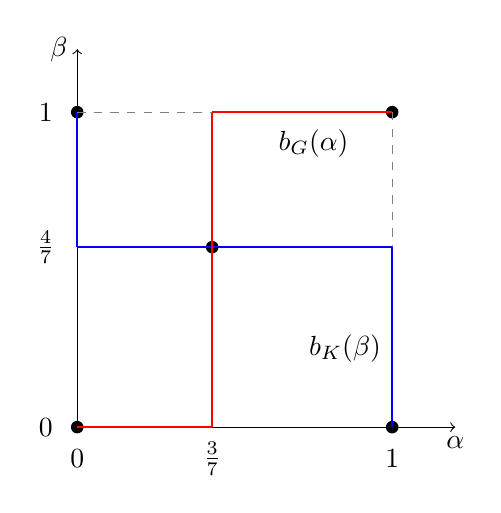
\begin{tikzpicture}[scale=4]
            % Axes
            \draw[->] (0,0) -- (1.2,0) node[below] {$\alpha$};
            \draw[->] (0,0) -- (0,1.2) node[left] {$\beta$};
        
            % Points
            \fill (0,0) circle (0.02); 
            \fill (0,1) circle (0.02); 
            \fill (1,0) circle (0.02); 
            \fill (1,1) circle (0.02); 
            \fill (3/7, 4/7) circle (0.02); 
        
            % Lines for best responses
            \draw[thick, blue] (0,1) -- (0, 4/7);
            \draw[thick, blue] (1,0) -- (1, 4/7);
            \draw[thick, blue] (0, 4/7) -- (1, 4/7);

            \draw[thick, red] (1,1) -- (3/7,1);
            \draw[thick, red] (0,0) -- (3/7, 0);
            \draw[thick, red] (3/7,0) -- (3/7,1);

            \draw[dashed, gray] (0, 1) -- (3/7,1);
            \draw[dashed, gray] (1, 1) -- (1, 4/7);
        
            % Labels
            \node at (0, -0.1) {$0$};
            \node at (3/7, -0.1) {$\frac{3}{7}$};
            \node at (1, -0.1) {$1$};
            \node at (-0.1, 0) {$0$};
            \node at (-0.1, 4/7) {$\frac{4}{7}$};
            \node at (-0.1, 1) {$1$};
            \node at (0.75, 0.9) {$b_G(\alpha)$};
            \node at (0.85, 0.25) {$b_K(\beta)$};
        
        \end{tikzpicture}
        \caption{Graph for $b_K(\beta)$ and $b_G(\alpha)$}
        \label{fig:best_response_1_2}
    \end{figure}

    As shown in Figure~\ref{fig:best_response_1_2}, the only NE is $\left\{\left(\frac{3}{7}, \frac{4}{7}\right), \left(\frac{4}{7}, \frac{3}{7}\right)\right\}$.

    Considering that there is a $25\%$ chance of the kicker missing when he chooses the right side, he will adjust his probability of kicking the ball to the right. However, he cannot adjust too much, or his opponent will be certain that he will kick to the right.

    Similarly, for the goalie, the benefit of defending the left side is higher because when he defends the left side, there is still a chance that the opponent might miss if they kick the ball to the right. Therefore, he will adjust the proportion of time he defends the left side accordingly.

    \section{Chicken Game}

    If both of them use pure strategy, it is easy to show that $(\mathcal{D}, \mathcal{S})$ and $(\mathcal{S}, \mathcal{D})$ are 2 NEs.

    If one plays mixed and the other plays pure strategy. WLOG, we let the row player play mixed strategy with probability $(\alpha, 1-\alpha)$, where $\alpha\in(0, 1)$. Now, if the column player plays $\mathcal{D}$, $U(\alpha)=1-\alpha$; if the column player plays $\mathcal{S}$, $U(\alpha)=-\alpha-5(1-\alpha)=4\alpha-5$. Both are linear functions, and we cannot find the maximum when $\alpha\in(0, 1)$. So there is no one pure one mixed NE.

    If both players play mixed strategy. Let the row player plays $(\alpha, 1-\alpha)$, the column player plays $(\beta, 1-\beta)$. By \textit{Indifference Principle}, we have:
    $$
    \begin{cases}
        -(1-\beta)=\beta-5(1-\beta)\\
        -(1-\alpha)=\alpha-5(1-\alpha)
    \end{cases}
    $$

    Solving this equation, we have:
    $$
    \alpha=\beta=\frac{4}{5}
    $$

    So all NEs are:
    $$
    \{(1, 0), (0, 1)\}, \{(0, 1), (1, 0)\}, \left\{\left(\frac{4}{5}, \frac{1}{5}\right),\left(\frac{4}{5}, \frac{1}{5}\right)\right\}
    $$

    \section{Who Doesn't Like Rock-Paper-Scissors}

    \subsection{NE in the Game}

    For Anna, $\mathcal{S}$ is strictly dominated by $\mathcal{R}$ (or $\mathcal{P}$). So we can remove it by \textit{Iterative Strict Dominance Elimination}.

    \[
    \begin{array}{|c|c|c|c|}
    \hline
     & \mathcal{R} & \mathcal{P} & \mathcal{S} \\ \hline
    \mathcal{R} & (0,0) & (-1,1) & (1,-1) \\ \hline
    \mathcal{P} & (1,-1) & (0,0) & (-1,1) \\ \hline
    \end{array}
    \]

    Then, we found that for Elsa, playing $\mathcal{R}$ is strictly dominated by playing $\mathcal{P}$. So we can remove the column $\mathcal{R}$. 

    \[
    \begin{array}{|c|c|c|c|}
    \hline
     & \mathcal{P} & \mathcal{S} \\ \hline
    \mathcal{R} & (-1,1) & (1,-1) \\ \hline
    \mathcal{P} & (0,0) & (-1,1) \\ \hline
    \end{array}
    \]

    We consider Anna plays $(\alpha, 1-\alpha)$ and Elsa plays $(\beta, 1-\beta)$. Same As Section~\ref{sec:football}, we define $U_A, U_E$ as the expected utility for Anna and Elsa, and $b_A, b_E$ as the correspondences of the best responses for Anna and Elsa.
    
    \begin{align*}
        U_A(\beta) &= -\alpha\beta+\alpha(1-\beta)-(1-\alpha)(1-\beta)\\
        &=2\alpha+\beta-3\alpha\beta-1\\
        &=\beta-1+(2-3\beta)\alpha\\
        U_E(\alpha) &= \alpha\beta-\alpha(1-\beta)+(1-\alpha)(1-\beta)+1\\
        &=3\alpha\beta-2\alpha-\beta+1\\
        &=(3\alpha-1)\beta-2\alpha+1
    \end{align*}

    So,
    \begin{align*}
        b_A(\beta)&=\begin{cases}
            \{1\}&\beta<\frac{2}{3}\\
            [0, 1]&\beta=\frac{2}{3}\\
            \{0\}&\beta>\frac{2}{3}
        \end{cases}\\
        b_E(\alpha)&=\begin{cases}
            \{0\}&\alpha<\frac{1}{3}\\
            [0, 1]&\alpha=\frac{1}{3}\\
            \{1\}&\alpha>\frac{2}{3}
        \end{cases}
    \end{align*}

    \begin{figure}[t]
    \centering
     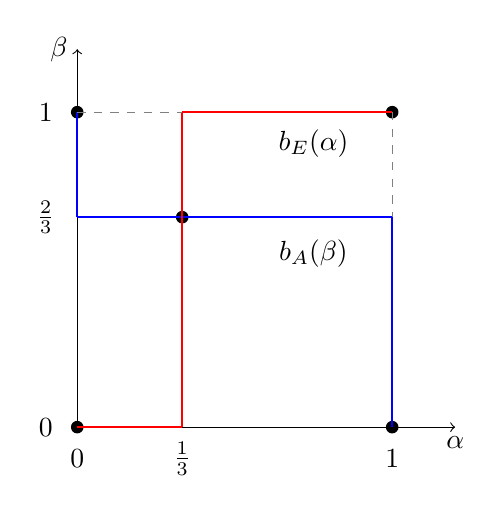
\begin{tikzpicture}[scale=4]
            % Axes
            \draw[->] (0,0) -- (1.2,0) node[below] {$\alpha$};
            \draw[->] (0,0) -- (0,1.2) node[left] {$\beta$};
        
            % Points
            \fill (0,0) circle (0.02); 
            \fill (0,1) circle (0.02); 
            \fill (1,0) circle (0.02); 
            \fill (1,1) circle (0.02); 
            \fill (1/3, 2/3) circle (0.02); 
        
            % Lines for best responses
            \draw[thick, blue] (0,1) -- (0, 2/3);
            \draw[thick, blue] (1,0) -- (1, 2/3);
            \draw[thick, blue] (0, 2/3) -- (1, 2/3);

            \draw[thick, red] (1,1) -- (1/3,1);
            \draw[thick, red] (0,0) -- (1/3, 0);
            \draw[thick, red] (1/3,0) -- (1/3,1);
            
            \draw[dashed, gray] (0, 1) -- (1/3,1);
            \draw[dashed, gray] (1, 1) -- (1, 2/3);
        
            % Labels
            \node at (0, -0.1) {$0$};
            \node at (1/3, -0.1) {$\frac{1}{3}$};
            \node at (1, -0.1) {$1$};
            \node at (-0.1, 0) {$0$};
            \node at (-0.1, 2/3) {$\frac{2}{3}$};
            \node at (-0.1, 1) {$1$};
            \node at (0.75, 0.9) {$b_E(\alpha)$};
            \node at (0.75, 0.55) {$b_A(\beta)$};
        
        \end{tikzpicture}
        \caption{Graph for $b_A(\beta)$ and $b_E(\alpha)$}
        \label{fig:best_response_3}
    \end{figure}

    In Figure~\ref{fig:best_response_3}, it is easy to find that the only NE is:
    $$\left\{\left(\frac{1}{3}, \frac{2}{3}\right), \left(\frac{2}{3}, \frac{1}{3}\right)\right\}$$.

    When we add the strategies we removed, the final answer is:
    $$
    \left\{\left(\frac{1}{3}, \frac{2}{3}, 0\right), \left(0, \frac{2}{3}, \frac{1}{3}\right)\right\}
    $$

    \subsection{Anna's Expected Playoff}
    
    The Anna's expected playoff is:
    $$
        U_A(\alpha, \beta) = 2\alpha+\beta-3\alpha\beta-1=-\frac{1}{3}
    $$

    \subsection{NE with Positive Probability}

    As the problem mentioned, both players play every strategy with a positive probability. We can let Anna plays $(\alpha, \beta, 1-\alpha-\beta)$, Elsa plays $(p, q, 1-p-q)$. Where
    $$0<\alpha, \beta, p, q, \alpha+\beta, p+q<1$$

    Then, by \textit{Indifference Principle}, we have:
    $$
    \begin{cases}
        -q+(1-p-q)=p-(1-p-q)=(-1-c)p+(1-c)q-c(1-p-q)\\
        -\beta+(1-\alpha-\beta)=\alpha-(1-\alpha-\beta)=-\alpha+\beta
    \end{cases}
    $$

    Solving this equation, we have
    \begin{align*}
    \begin{cases}
        \alpha=\frac{1}{3}\\
        \beta=\frac{1}{3}
    \end{cases}&
    \begin{cases}
        p=\frac{1-c}{3}\\
        q=\frac{1+c}{3}
    \end{cases}
    \end{align*}

    So the Nash Equilibrium is:
    $$
    \left\{\left(\frac{1}{3}, \frac{1}{3}, \frac{1}{3}\right), \left(\frac{1-c}{3}, \frac{1+c}{3}, \frac{1}{3}\right)\right\}
    $$

    \section{Nash Equilibrium for 3 by 3 Game}

    \subsection{Pure Nash Equilibrium}

    We define $b(\cdot)$ as the set of best responses.

    For the row player:

    $$
    \begin{cases}
        b(\mathcal{L})=\{\mathcal{B}\}\\
        b(\mathcal{C})=\{\mathcal{T}, \mathcal{M}\}\\
        b(\mathcal{R})=\{\mathcal{M}\}
    \end{cases}
    $$

    For the column player:

    $$
    \begin{cases}
        b(\mathcal{T}) = \{\mathcal{L}\}\\
        b(\mathcal{M}) = \{\mathcal{C}\}\\
        b(\mathcal{B}) = \{\mathcal{R}\}
    \end{cases}
    $$

    So we can find that $(\mathcal{M}, \mathcal{C})$ is the only pure NE for this game.

    \subsection{All Mixed Nash Equilibria with a Support I}

    Let the row player plays $(\alpha, \beta, 1-\alpha-\beta)$, column player plays $(p, q, 1-p-q)$.

    Then, by \textit{Indifference Principle}, we have:
    $$
    \begin{cases}
        q+2(1-p-q)=-p+q+3(1-p-q)=p-2q+2(1-p-q)\\
        4\alpha+2\beta+3(1-\alpha-\beta)=2\alpha+3\beta+(1-\alpha-\beta)=\beta+8(1-\alpha-\beta)
    \end{cases}
    $$

    By solving this, we can get:
    \begin{align*}
    \begin{cases}
        \alpha=\frac{1}{9}\\
        \beta=\frac{2}{3}
    \end{cases}&
        \begin{cases}
            p=\frac{3}{7}\\
            q=\frac{1}{7}
        \end{cases}
    \end{align*}

    So the NE is
    $$
    \left\{\left(\frac{1}{9}, \frac{2}{3}, \frac{2}{9}\right), \left(\frac{3}{7}, \frac{1}{7}, \frac{3}{7}\right)\right\}
    $$

    \subsection{All Mixed Nash Equilibria with a Support II}

    Let the row player play $(\alpha, 1-\alpha, 0)$.

    As $b(\mathcal{C})=\{\mathcal{T}, \mathcal{M}\}$. We only need to satisfy:

    $$
    \mathcal{C}\in b_{\text{column player}}(\{\mathcal{T}: \alpha; \mathcal{M}: 1-\alpha; \mathcal{B}: 0\})
    $$

    So
    $$
    \begin{cases}
        2\alpha+3(1-\alpha)\ge 4\alpha+2(1-\alpha)\\
        2\alpha+3(1-\alpha)\ge 1-\alpha
    \end{cases}
    $$

    So we need $0<\alpha\le \frac{1}{3}$.

    So all $(\alpha, 1-\alpha, 0)$ with $0<\alpha\le\frac{1}{3}$ are NEs to the game.
\end{document}
